\section{Video segmentation for event extraction}

\subsection{SVM based approach}

Our first approach is training a SVM linear classifier. We believe that the distributions of colors in the image provides a great deal of information about whether the image corresponds to an indoor or outdoor scene, so we have use a sampled down version of the histogram as the SVM's input. More specifically we have obtained for each image all the channels' histograms with only 5 bins. This means that for each image we have a total of 15 features. Also, in order to train the SVM we had to tag the images manually (see annex for more details)
\footnote{Suggestion: for next years provide the students with the correct tags for each image, so their approaches (even if they are not based on a Machine Learning technique) can be tested against a decent number of images and not just a few ones. We offer our tags if they are of any value (they are stored in the \texttt{GroundTruth.mat} file).}.

We have taken a random sample of 100 images for training and the 117 remaining ones were left for testing. After training our classifier and testing it against the test images we have obtained an accuracy of about an 83.76\% which is actually a quite good result. For completeness, we show the confusion matrix in table \ref{tab:confusion-matrix}. As we can see, the problem is not unbalanced and the classifier is not particularly biased towards predicting \emph{Indoor} or \emph{Outdoor}.

Figure \ref{fig:svm-graphical-results} shows some examples of correct and bad guesses. We believe that what causes the classifier to miss in figure \ref{fig:indoor-failed} is the intense glare at the top left corner, while the reason behind the misclassification in \ref{fig:outdoor-failed} is that the sky is obstructed by a tree which is much darker.

The relevant code for this strategy is located at \texttt{tag\_images.m}, \texttt{svm\_train\_and\_test.m} and \texttt{demo\_svm.m}. The files \texttt{GroundTruth.mat}, \texttt{Features-s42.mat} and \texttt{SVMModel.mat} contain precached variables. See the annex for more details.

\begin{table}[htb]
\centering
\begin{tabular}{l|rr}
\textbf{Guess{\textbackslash}Truth} & \textbf{Indoor} & \textbf{Outdoor} \\ \hline
\textbf{Indoor} & 52 & 13 \\
\textbf{Outdoor} & 6 & 46 \\
\end{tabular}
\caption{Confusion matrix of the SVM classifier}
\label{tab:confusion-matrix}
\end{table}

\begin{figure}[htb]
	\centering
	\begin{subfigure}[t]{0.4\textwidth}
		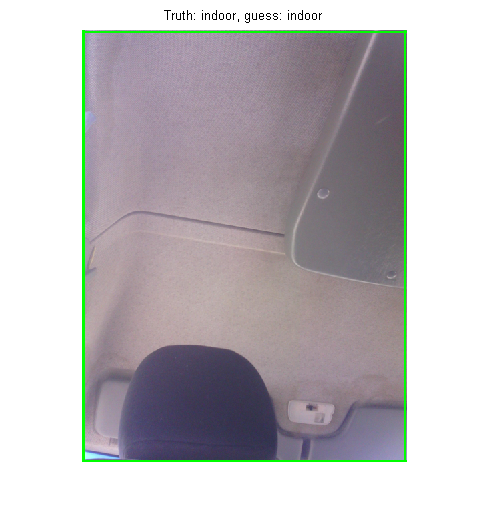
\includegraphics[width=\textwidth]{./img/ex2/indoor-nailed.png}
		\caption{Indoor scene correctly recognized}
		\label{fig:indoor-nailed}
	\end{subfigure}
	~
	\begin{subfigure}[t]{0.4\textwidth}
		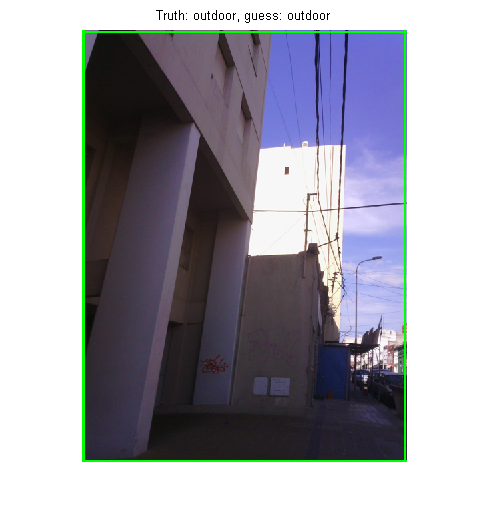
\includegraphics[width=\textwidth]{./img/ex2/outdoor-nailed.png}
		\caption{Outdoor scene correctly recognized}
		\label{fig:outdoor-nailed}
	\end{subfigure}
	
	\begin{subfigure}[t]{0.4\textwidth}
		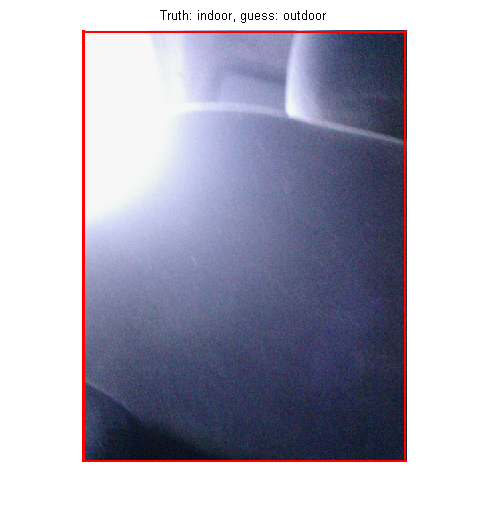
\includegraphics[width=\textwidth]{./img/ex2/indoor-failed.png}
		\caption{Failure recognizing indoor scene}
		\label{fig:indoor-failed}
	\end{subfigure}
	~
	\begin{subfigure}[t]{0.4\textwidth}
		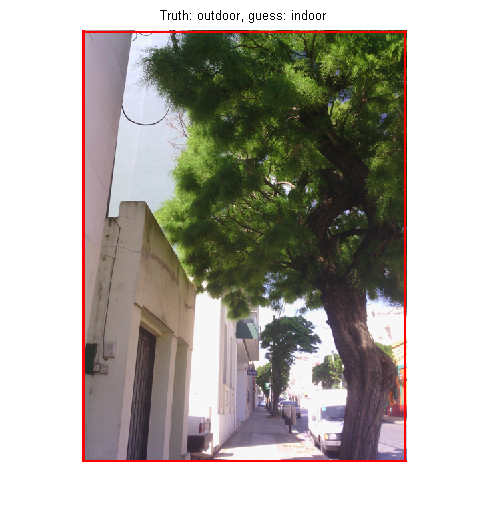
\includegraphics[width=\textwidth]{./img/ex2/outdoor-failed.png}
		\caption{Failure recognizing outdoor scene}
		\label{fig:outdoor-failed}
	\end{subfigure}
	
\caption{Some examples of correct and incorrect guesses with our SVM classifier}
\label{fig:svm-graphical-results}
\end{figure}
